\documentclass[12pt]{amsart}

\addtolength{\hoffset}{-2.25cm}
\addtolength{\textwidth}{4.5cm}
\addtolength{\voffset}{-2.5cm}
\addtolength{\textheight}{5cm}
\setlength{\parskip}{0pt}
\setlength{\parindent}{15pt}
\usepackage{listings}
\usepackage{amsthm}
\usepackage{amsmath}
\usepackage[spanish]{babel}
\usepackage[sort&compress, numbers]{natbib}
\usepackage{amssymb}
\usepackage[utf8]{inputenc}
\usepackage[colorlinks = true, linkcolor = magenta, citecolor = magenta, final]{hyperref}
\usepackage{listings}
\usepackage{ragged2e}
\usepackage{subcaption}

\usepackage{graphicx}
\usepackage[sort&compress, numbers]{natbib}
\usepackage{xcolor}
\usepackage{listings}
\usepackage{ragged2e}

\usepackage{graphicx}
\usepackage[sort&compress, numbers]{natbib}
\usepackage{xcolor}
\usepackage{listings}
\usepackage{ragged2e}
\hypersetup{
    colorlinks=true,
    linkcolor=magenta,
    filecolor=magenta,     
    urlcolor=magenta,
}
\usepackage{graphicx}
\usepackage[sort&compress, numbers]{natbib}
\usepackage{xcolor}
\usepackage{listings}
\usepackage{ragged2e}

\lstset{style=mystyle}
\usepackage{graphicx}
\usepackage{multicol}
\usepackage{ marvosym }
\newcommand{\ds}{\displaystyle}


\pagestyle{myheadings}

\setlength{\parindent}{0in}
\begin{document}

\pagestyle{empty}



\thispagestyle{empty}

{\scshape Simulación} \hfill {\scshape \Large Tarea 4: Diagramas de Voronoi} \hfill  {\scshape 09/Mar/2021}
\author{C. María Montemayor Palos}
\maketitle

\hrule
\hrule
\bigskip


\section{Objetivo}
El objetivo es examinar de manera sistemática el efecto del número de semillas y del tamaño de la zona en la distribución en las grietas que se forman en términos de la mayor distancia manhattan entre la grieta y el exterior de la pieza \cite{dra}.


\section{Metodología}
Se utilizó el programa R versión 4.0.4 \cite{R} para Windows llevando así a cabo la ejecución de la tarea asignada. En el experimento, se considera primeramente el tamaño de la pieza como $n\times n$, donde $n \in \lbrace 40, 60, 80, 100\rbrace$. Posteriormente se colocan las semillas al azar $k$, donde $k$ \in \{12, 22, 32, 42\}$ por cada combinación realizándola un total de 200 veces. Una vez generado el tamaño de la pieza y colocadas las semillas, se propaga la grieta dentro de la pieza, con una mayor probabilidad de que se produzca en la frontera y con una menor probabilidad de que crezca hacia el centro. Finalmente se calcula la distancia manhattan máxima del borde de la grieta hacia el centro. El código está basado mayormente, en el código implementado por Schaeffer E. \cite{dracodigo}. Finalmente se genera el gráfico de caja-bigote para la comparación de los resultados.

\section{Código}
Se determinan los tamaños de las piezas y la cantidad de semillas.
\begin{lstlisting}
largos=data.frame()
dim<-  seq(40, 100, by=20)
sem<-seq(12, 42, by=10)

for (n in dim) {
  for (k in sem) {
      zona <- matrix(rep(0, n * n), nrow = n, ncol = n)
\end{lstlisting}
\bigskip
Posteriormente se calcula la distancia manhattan máxima de la grieta.
\begin{lstlisting}
manhattan=function(largo){return(sum(abs((i[1]-xg)-(i[2]-yg))))}
      return(largo)
\end{lstlisting}

\section{Resultados y discusión}
En la figura \ref{fig1} se muestra un ejemplo de las celdas de Voronoi, en una zona de distribución de $100\times100$ para 22 semillas con su respectiva grieta formada. Se puede apreciar que la figura \ref{fig2} tiene también una zona de distribución de $100\times100$ con 42 semillas, es decir, casi el doble de semillas. Comparando ambas figuras, se puede apreciar que no varía mucho el tamaño de la grieta hacia el centro en función de las semillas.
\newpage
\begin{figure}
\centering
\begin{subfigure}[b]{0.3\linewidth}
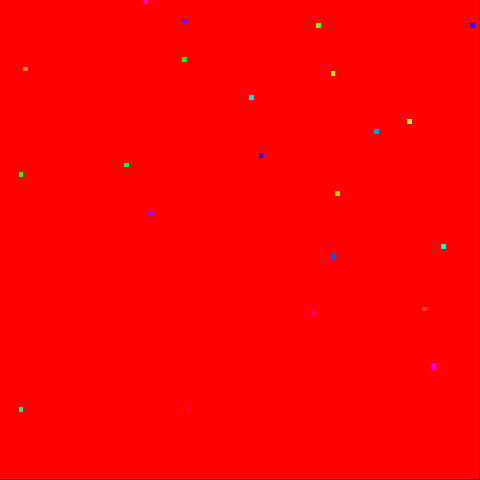
\includegraphics[width=\linewidth]{p4s-22.png}
\caption{Semillas distribuidas.}
\label{o}
\end{subfigure}
\begin{subfigure}[b]{0.3\linewidth}
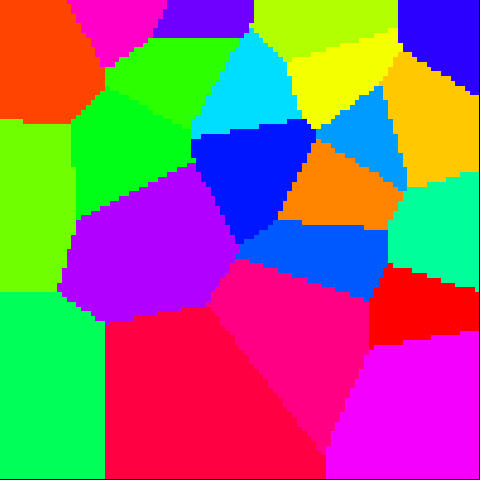
\includegraphics[width=\linewidth]{p4c-22.png}
\caption{Celdas formadas.}
\label{s}
\end{subfigure}
\begin{subfigure}[b]{0.3\linewidth}
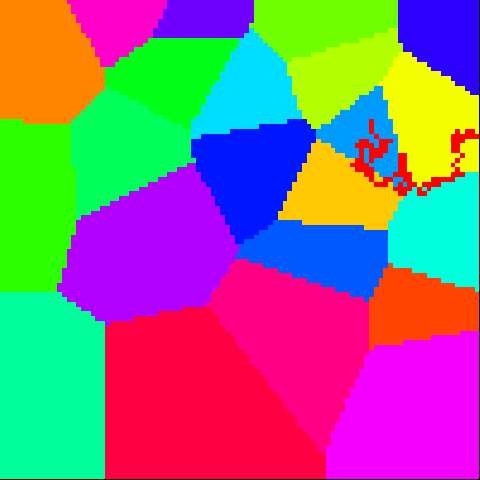
\includegraphics[width=\linewidth]{p4g_91.png}
\caption{Grieta formada.}
\label{se}
\end{subfigure}
\caption{Zona de $100\times100$ para 22 semillas.}
\label{fig1}
\end{figure}

\begin{figure}
\centering
\begin{subfigure}[b]{0.3\linewidth}
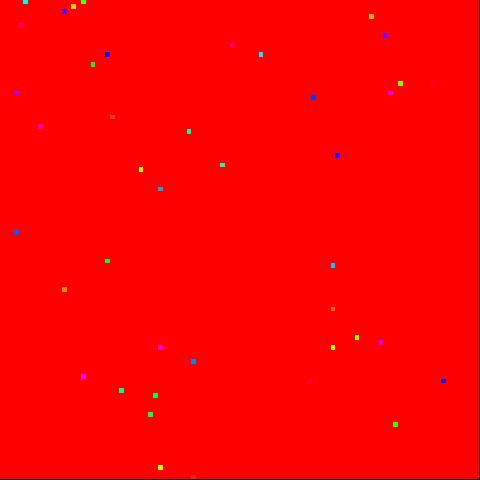
\includegraphics[width=\linewidth]{p4s-42.png}
\caption{Semillas distribuidas.}
\label{o}
\end{subfigure}
\begin{subfigure}[b]{0.3\linewidth}
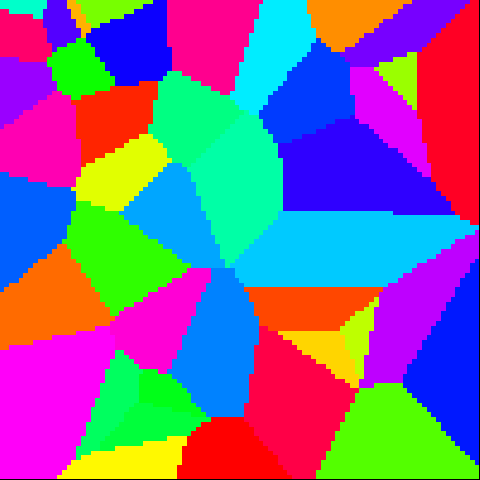
\includegraphics[width=\linewidth]{p4c-42.png}
\caption{Celdas formadas.}
\label{s}
\end{subfigure}
\begin{subfigure}[b]{0.3\linewidth}
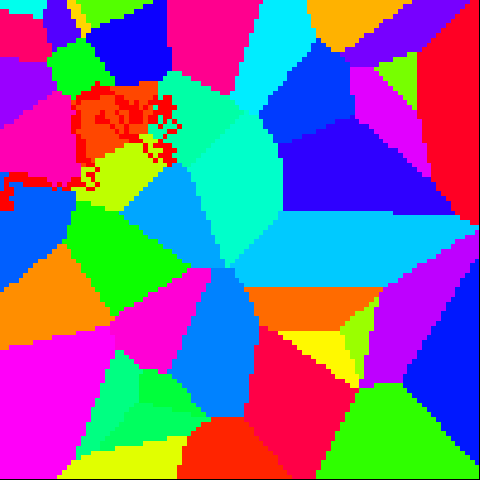
\includegraphics[width=\linewidth]{p4g_40.png}
\caption{Grieta formada.}
\label{se}
\end{subfigure}
\caption{Zona de $100\times100$ para 42 semillas.}
\label{fig2}
\end{figure}
Los datos generales obtenidos del total de piezas rotas se muestran en el cuadro \ref{datos1}.
\bigskip
\bigskip
\begin{table}[ht]
    \caption{Fragmento de los datos recopilados del experimento}
    \label{datos1}
    \centering
    \begin{tabular}{|r|r|r|}
       \hline
        Tamaño&Semillas&Piezas rotas\\
        \hline
        $40\times40$ & 12 & 8 \\
        $60\times60$ & 22 & 7 \\
        $80\times80$ & 32 & 7 \\
        $100\times100$ & 42 & 2 \\
        \hline
    \end{tabular}
\end{table}
\bigskip


En la figura \ref{fig3} se observan los diagramas de caja-bigote para cada cantidad de semillas y de zonas, se aprecia que a mayor tamaño de zona, mayor será el acercamiento de la grieta generada al centro.
\newpage
\begin{figure}
    \centering
    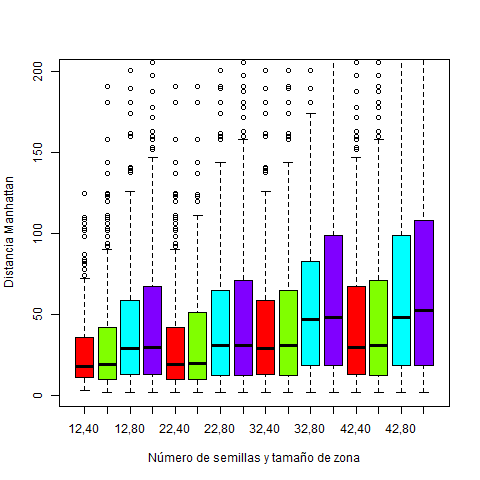
\includegraphics[width=0.5\textwidth]{totaldiagramas.png}
    \caption{Diagrama caja bigote de las distancias manhattan máximas variando el número de semilla y el tamaño de la zona de distribución de la celda de Voronoi respectivamente.}
    \label{fig3}
\end{figure}
Se generó también una gráfica de las densidades de todas las grietas formadas (ver figura \ref{fig4}).
\begin{figure}
    \centering
    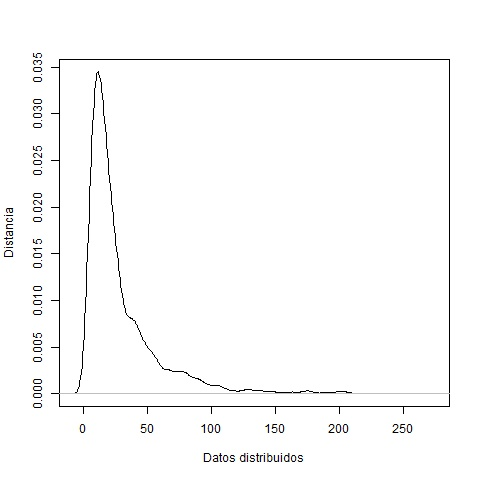
\includegraphics[width=0.5\textwidth]{densidad.jpg}
    \caption{Densidad de las grietas formadas.}
    \label{fig4}
\end{figure}
\newpage
\section{Conclusión}
Se concluye que la cantidad de semillas distribuídas no afecta en gran medida a la pieza, lo que provoca su fractura es el tamaño de la zona, a menor tamaño será mayor la probabilidad de generarse una grieta.
\bigskip

\bibliography{referencias}
\bibliographystyle{plainnat}


\bigskip

\end{document}
